\chapter{Cross Plattform Frameworks}
Für die Realisierung eine Source-to-Source Compilers gibt es zwei relevante Faktoren,  die für die Realisierung ausschlaggebend sind.  Zum einen die Programmiersprachen in dem die beiden Frameworks entwickelt werden,  da bei der Übersetzung eine Brücke zwischen Quell und Zielsprache geschlagen werden muss.  Neben der Programmiersprache ist jedoch auch die Arbeitsweise eines Frameworks von essentieller Bedeutung.  Wie die Definition von Compilern bereits einführte,  müssen die Programme vor und nach der Übersetzung gleichwertig sein.  Dies implementiert,  dass das Verhalten der übersetzten Anwendungen nach der Übersetzung identisch seien muss wie das der Ursprungsanwendung.  Es ist also notwendig,  neben den sprachlichen auch die technischen Unterschiede zwischen den Frameworks zu kennen und diese im Rahmen der compilierung zu optimieren. 

\section{Frameworks}
Xamarin is eine Open Source-Plattform für das Erstellen mobiler Anwendungen für iOS und Android mit Hilfe des .NET Frameworks, welches von Microsoft weiterentwickelt wird.  Dabei ist Xamarin ist eine Abstraktionsebene, die die Kommunikation zwischen Code und dem zugrunde liegenden Plattformcode verwaltet.  Xamarin wird in einer verwalteten Umgebung ausgeführt, die Vorteile wie Speicherbelegung und Garbage Collection bietet.  Bei Xamarin.Forms handelt es sich um ein Open-Source-Benutzeroberflächenframework., mit dessen Hilfe Entwickler iOS- und Android-Anwendungen aus einer einzigen CodeBase erstellen können.  Dabei wird auf die in der .NET Welt bekannten Technologien XAML  für die Benutzeroberfläche und C\# für die Anwendungslogik zurückgegriffen.  Die einzelnen Benutzeroberflächen werden von Xamarin.Forms als native Steuerelemente auf jeder Plattform gerendert.  \footcite[Vgl.][Abgerufen am 28.10.2020]{MicrosoftWhatIsXam2020}

Flutter ist ebenfalls wie Xamarin.Forms ein Open Source Framework für die Erstellung von 2D mobilen Anwendungen.  Dabei werden im Vergleich zu Xamarin.Forms keine nativen Steuerelemente für jede Plattform gerendert sondern beinhaltet eine Sammlung von so genannten Widgets, die von dem Framework vewaltet und gerendert werden.  Für die Anzeige dieser Widgets wird auf die 2D engine Skia zugegriffen.  Flutter geht diesen Weg,  da das Endergebnis der Anwendungen eine höhere Qualität verspricht, da die nativen Steuerelemente in Bezug auf Flexibilität und Qualität begrenzt sind.  Außerdem ist es durch die Verwendung derselben Renderes einfacher, von derselben Codebasis aus für mehrere Plattformen zu veröffentlichen,  ohne eine sorgfältige und kostspielige Planung vornehmen zu müssen,  um verschiedene Funktionssätze und API-Merkmale aufeinander abzustimmen.\footcite[Vgl.][Abgerufen am 28.10.2020]{GoogleFlutterFAQ2020}

Dieser essentielle Unterschied zwischen den Frameworks werden in den folgenden Abschnitten dieser Arbeit deutlicher und sind bei der Übersetzung der Anwendungen fokussiert zu Berücksichtigen. 
\subsection{Projekte}
Xamarin.Forms Projektmappen setzen sich aus mehreren Projekten zusammen.  Zwei Projekten für jeweils iOS und Android,  welche den plattformspezifischen Code beinhalten sowie ein zusätzliches für den Quelltext,  der zwischen den Plattformen geteilt wird.  Im Gegensatz dazu gibt es bei Flutter nur ein Projekt, welches alle notwendigen Inhalte für iOS und Android beinhaltet.  Xamarin.Forms bietet Entwicklern die Möglichkeit über die plattformbezogenen Projekte die nativen Renderer zu manipulieren.  Durch diese sogenannten Custom Renderer (deutsch: benutzerdefinierter Renderer)ist es möglich unterschiedliche Darstellungen und Verhalten je nach Plattform zu erzeugen.  Flutter bietet diese Möglichkeit nicht, da wie bereits beschrieben ausschließlich einheitliche Renderer Angeboten werden. 

\subsection{Views}
Views (zu Deutsch Ansichten) sind visuelle Elemente die in zwei Kategorien unterschieden werden können.  Controls, die für die Sammlung von Benutzereingaben oder die Ausgabe von Daten sind.  Sowie Layouts die eine Sammlung von Ansichten beinhalten und für die Anordnung der untergeorderten Ansichten in der Benutzeroberfläche verantwortlich sind. Außerdem arbeitet sie mit jeder untergeordneten Ansicht zusammen, um die endgültige Rendering-Größe zu bestimmen.\footcite[Vgl.][Abgerufen am 28.10.2020]{Ritscher2020}
\subsubsection{Pages}
Pages (zu Deutsch: Ansichtseiten) sind visuelle Elemente einer Anwendung die den gesamten Bildschirm belegen und zu den Layout Views gehören.  Xamarin Forms bietet dafür 
verschiedene Alternativen an,  die in \ref{fig:Xamarin.Forms Pages} grafisch dargestellt sind.\footcite[Vgl.][Abgerufen am 28.10.2020]{MicrosoftXamPages2016}

\begin{figure}[h]
 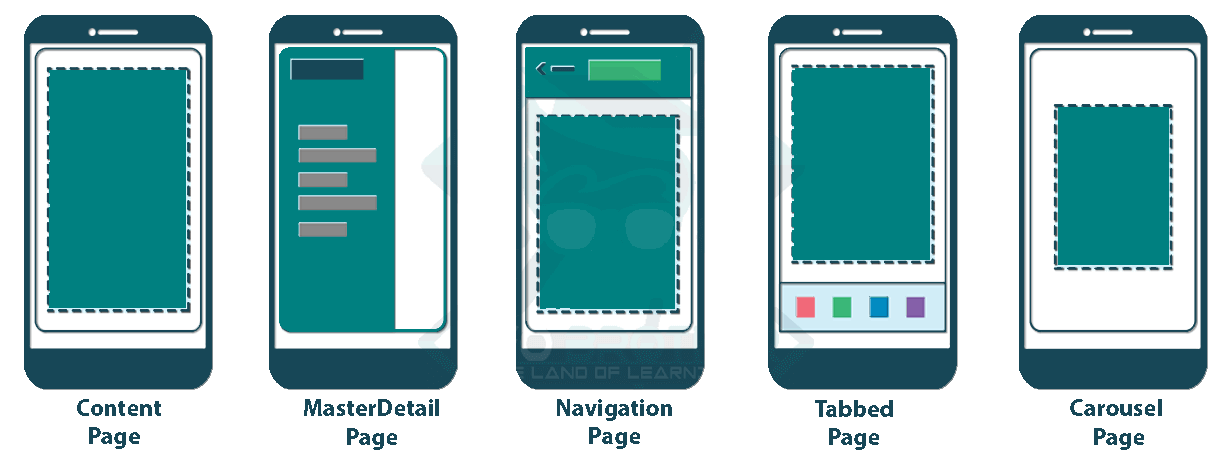
\includegraphics[width=\textwidth,height=\textheight,keepaspectratio]{Images/CrossPlattformFrameworks/XamarinPages.png}
 \caption{Xamarin.Forms Pages}
 \label{fig:Xamarin.Forms Pages}
\end{figure}

Wie die Darstellung präsentiert, hat die Auswahl einer Page einen direkten Einfluss auf das Navigationskonzept innerhalb der Anwendung.  Abgesehen von der ContentPage, die ausschließlich eine View anzeigt haben die jeweiligen Seiten die folgende Navigation zur folge: 

\begin{itemize}
 \item FlyOutPage: Eine Seite, die zwei Bereiche für die Seite hat. Typischerweise enthält das Flyout ein Menü über welches zwischen den eigentlichen Inhaltsseiten navigiert werden kann.
 \item NavigationPage: Eine Seite, die eine Navigationsleiste enthält.  Die Seiten werden auf einem Stapel gehalten und es kann zwischen ihnen gesprungen werden.  Die Navigationsleiste kann sowohl Navigationsschaltflächen als auch einen Titel enthalten.
 \item TabbedPage: Eine Container-Seite.  Die TabbedPage fungiert als Container,  der die mit jeder Registerkarte verbundenen Inhaltsseiten enthält.
\end{itemize}


Die Auswahl einer Page hat daher bei Xamarin Forms einen direkten Einfluss auf die Navigation durch die Anwendung.  

%Flutter gibt es alternativ weniger Auswahl, da lediglich ein "MaterialApp" und eine "CupertinoApp" als Widget zur Verfügung stellen und alternativ Materialdesign oder Cupertino design anbieten. 
%Um Seiten mit Tab oder einem Slideout zu genierieren bietet Flutter jedoch ebenfalls Widgets an. 
\subsubsection{Elemente}
\subsubsection{Layouts}
\subsubsection{Listen}
\subsubsection{Gesten}
\subsubsection{Animtion}

\subsection{Navigation}
Pages.
Andere Apps
\subsection{Async UI}
\subsection{Netzwerk Anfragen}
\subsection{Abhängigkeiten}
\subsection{Lebenzyklus}
\subsection{Schriften}
\subsection{Plugins}
Interacting with hardware, third party services, and the platform
\subsection{Databases and locale storage}
\subsection{Notifications}
\section{Programmiersprachen}
C\# Dart Vergleich
XAML Dart

